\section{基本介绍}

本节将一步步展示如何安装配置本集成工具。

\begin{figure}[H]
    \Centering
    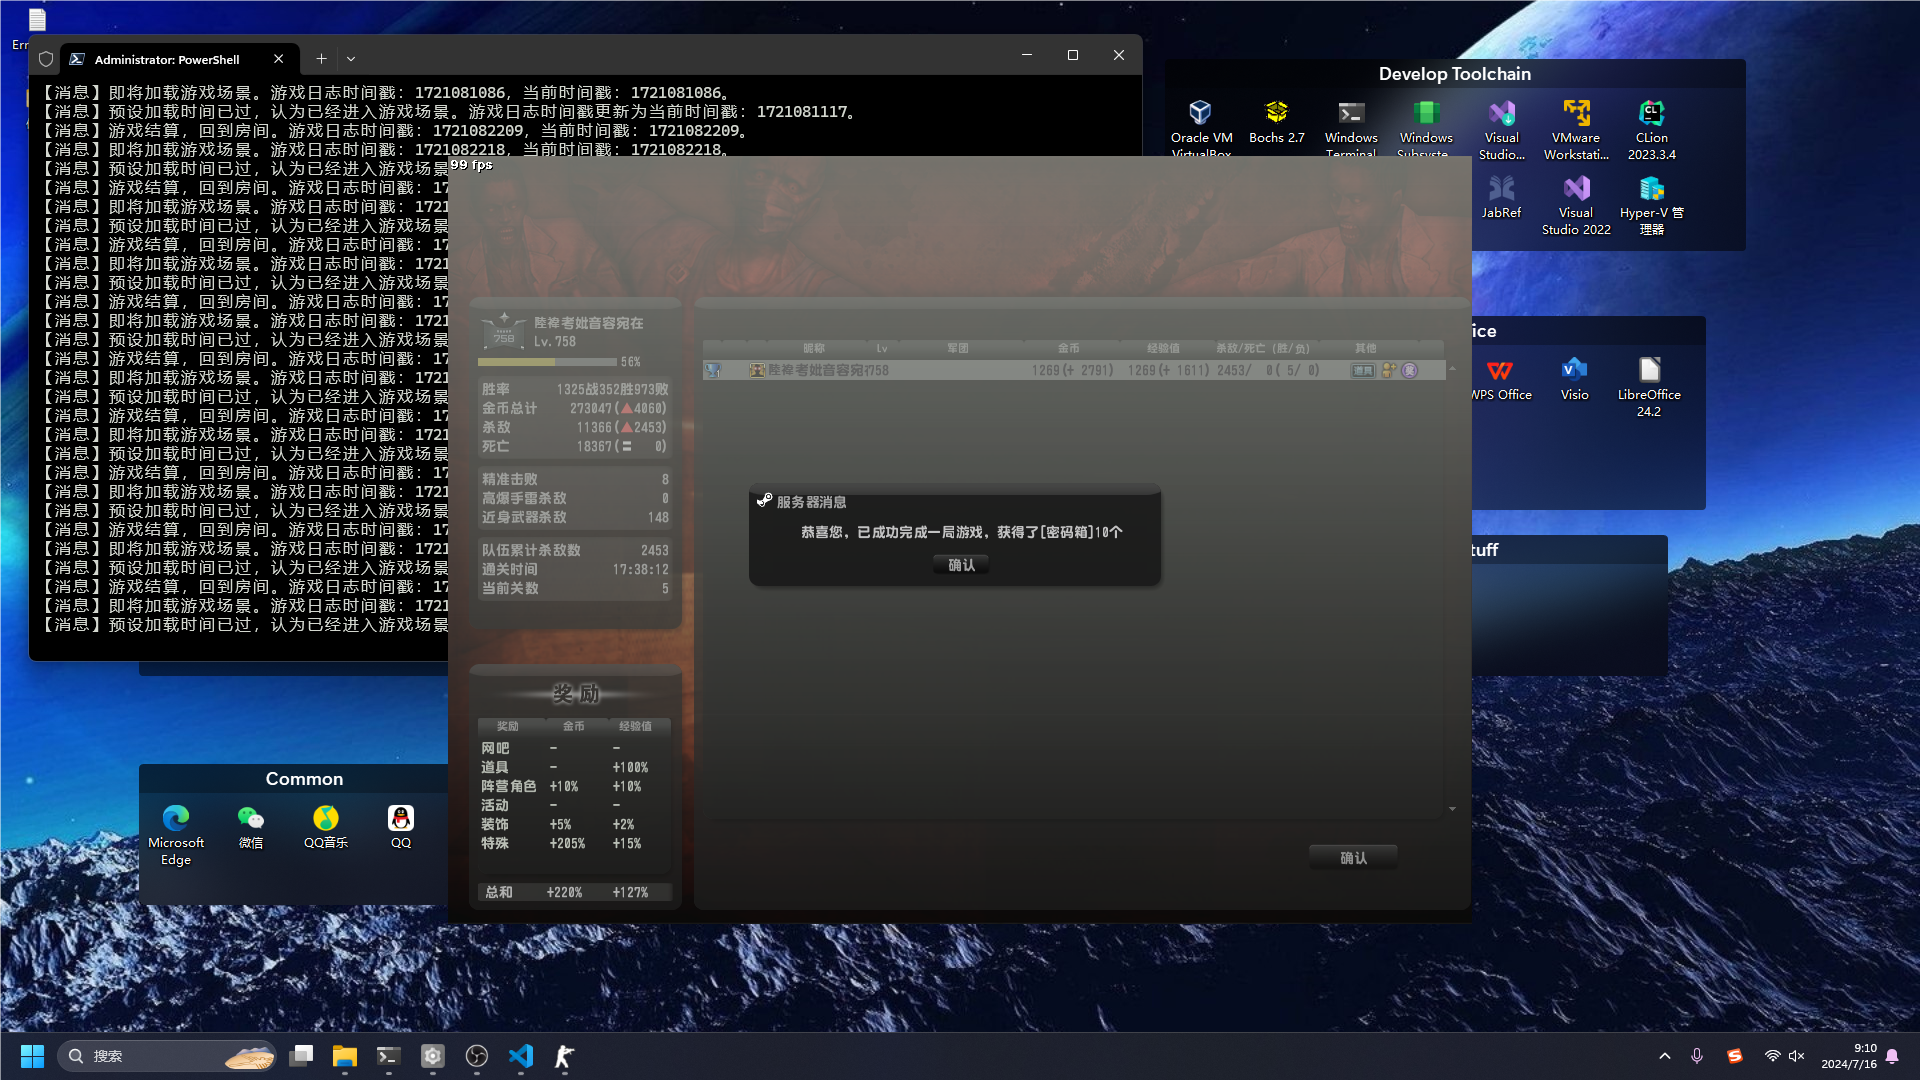
\includegraphics[width=\textwidth]{docs/assets/controller.png}
    \caption{运行效果展示}
\end{figure}

\subsection{罗技软件导入 LUA 程序}

将压缩包解压,\textbf{\color{red}解压路径不能包含非英文字符},否则 LUA 脚本无法运行。

鼠标右键点击 \lstinline{install.ps1} 点击在 Powershell 中运行,完成对 LUA 程序的配置。

配置完成后,如果变动了安装路径,则需要重新运行一次 \lstinline{install.ps1},并重新在罗技软件中保存并运行(详见下文)。

\begin{figure}[H]
    \Centering
    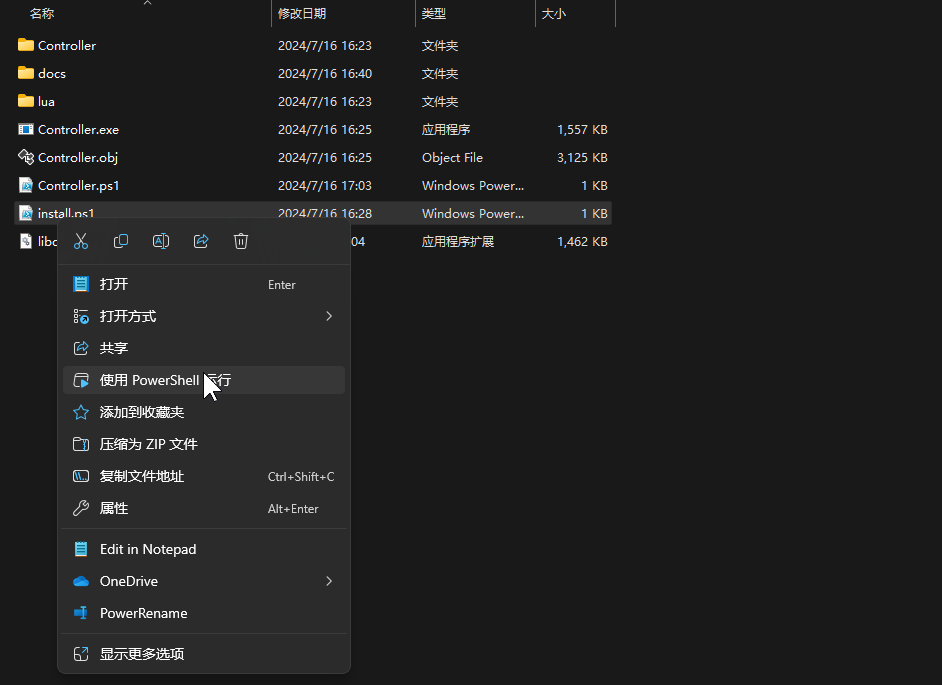
\includegraphics[width=\textwidth]{docs/assets/install.png}
    \caption{运行 \lstinline{install.ps1}}
\end{figure}

然后,前往罗技官网下载安装最新版的 Logitech G HUB 软件。\textbf{\color{red}不需要您拥有任何的罗技硬件设备。}

安装并\textbf{\color{red}以管理员权限}启动 Logitech G HUB 软件。否则会因为权限问题导致游戏无法正确接收软件发出的键鼠消息。

\begin{figure}[H]
    \Centering
    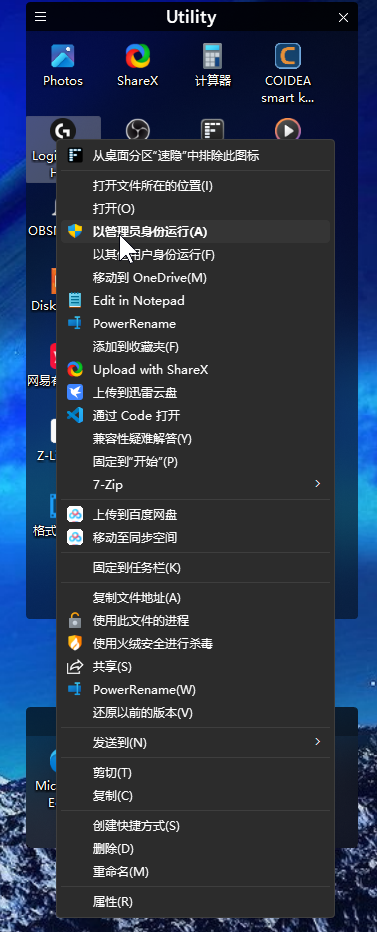
\includegraphics[width=\textwidth]{docs/assets/run_lghub.png}
    \caption{以管理员权限运行 Logitech G HUB}
\end{figure}

可以右键 Logitech G HUB 快捷方式,点击“属性”。在对话框中点击“高级”,选中“用管理员身份运行”后确认,这样就不必每次都右键以管理员权限启动了。

\begin{figure}[H]
    \Centering
    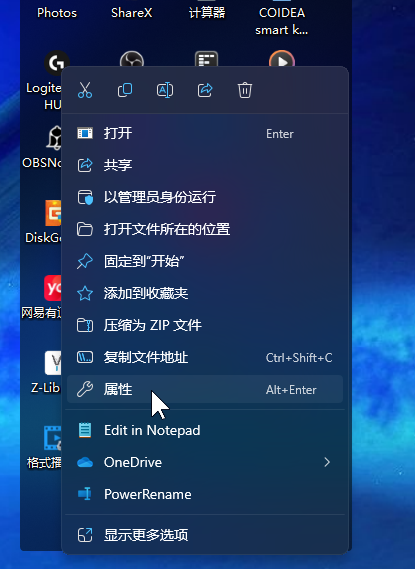
\includegraphics[width=\textwidth]{docs/assets/lghub_property.png}
    \caption{点击“属性”}
\end{figure}

\begin{figure}[H]
    \Centering
    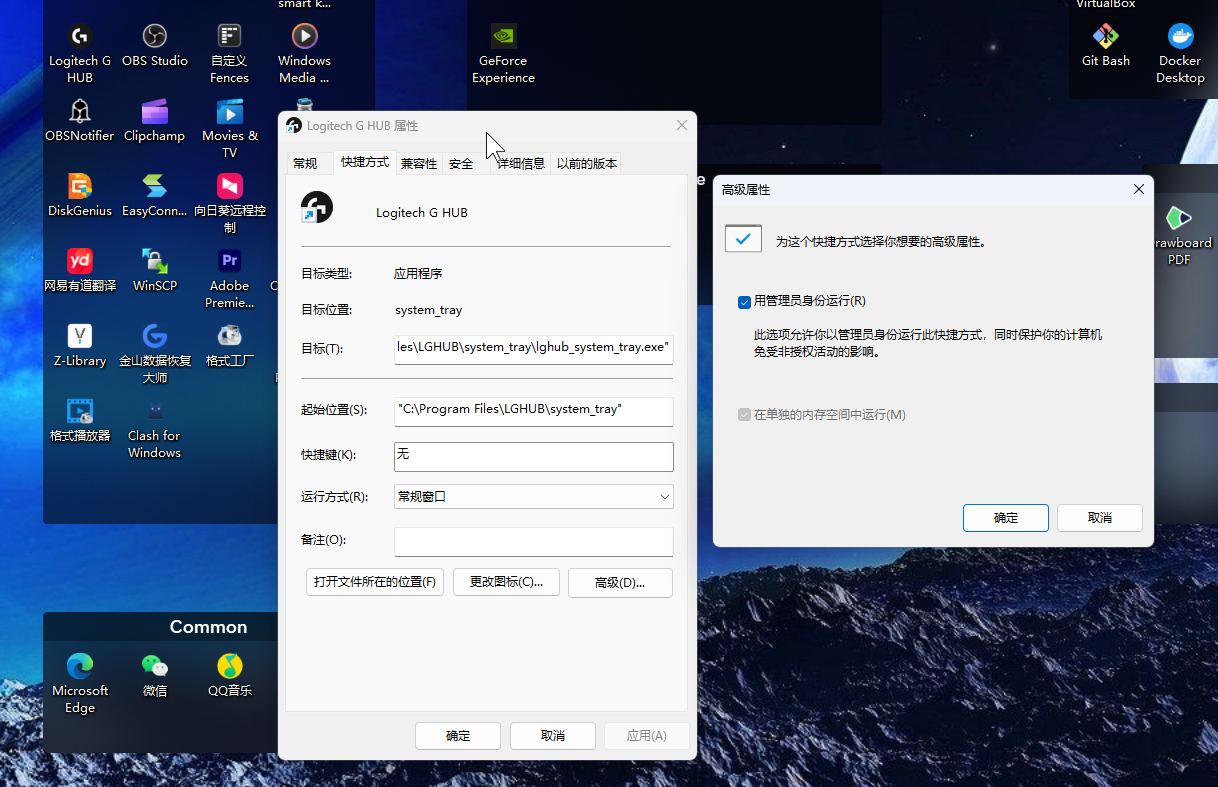
\includegraphics[width=\textwidth]{docs/assets/lghub_advanced.png}
    \caption{点击“高级”,并选中“用管理员身份运行”}
\end{figure}

需要注意,Logitech G HUB 有时会自动更新。更新后快捷方式需要重新设置为“用管理员身份运行”。

\begin{figure}[H]
    \Centering
    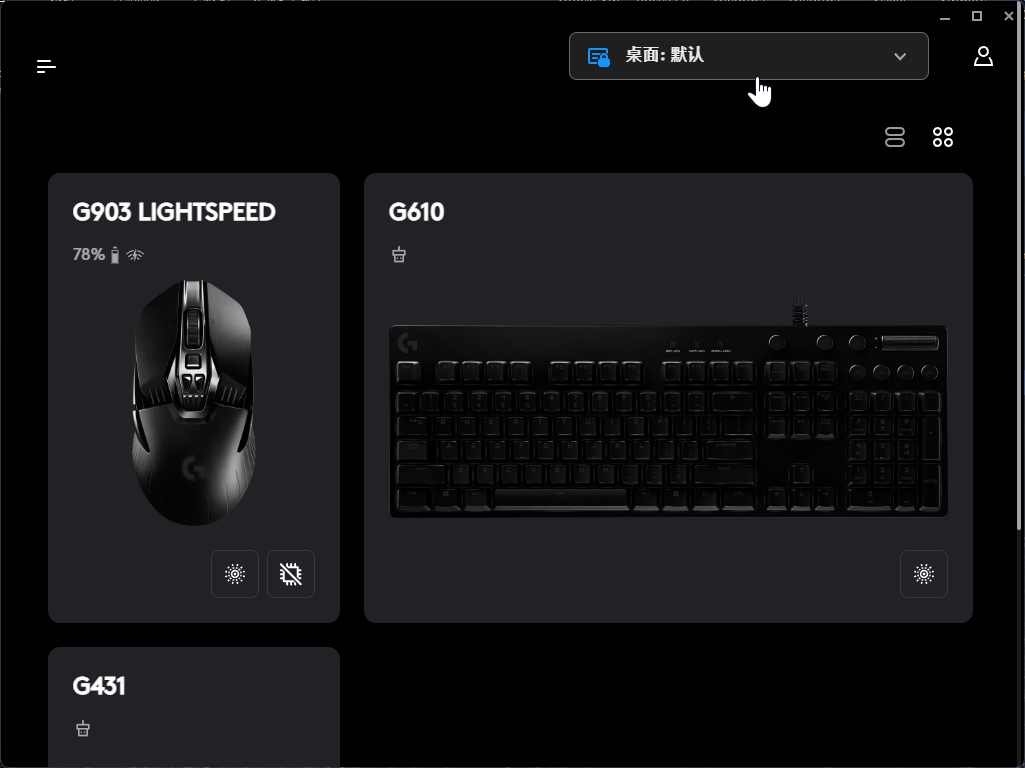
\includegraphics[width=\textwidth]{docs/assets/lghub.png}
    \caption{Logitech G HUB 软件}
\end{figure}

进入界面后,点击软件上方下拉框,选择“管理配置文件”。

\begin{figure}[H]
    \Centering
    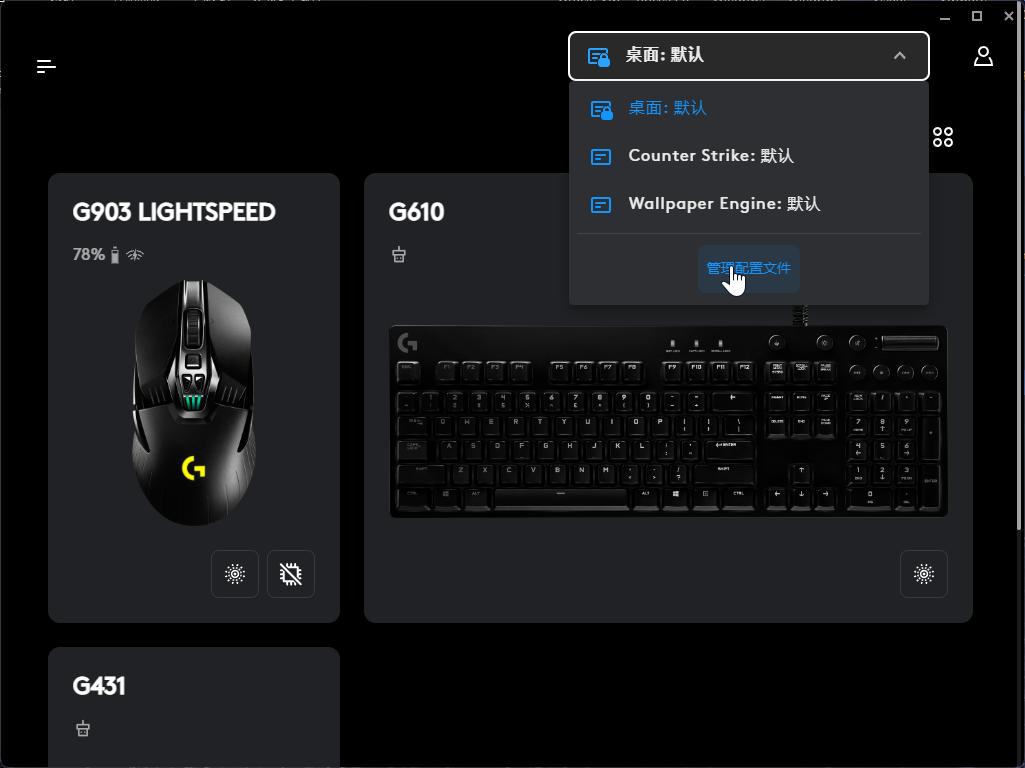
\includegraphics[width=\textwidth]{docs/assets/manage_configs.png}
    \caption{点击“管理配置文件”}
\end{figure}

在下一级界面中点击“编写脚本”。

\begin{figure}[H]
    \Centering
    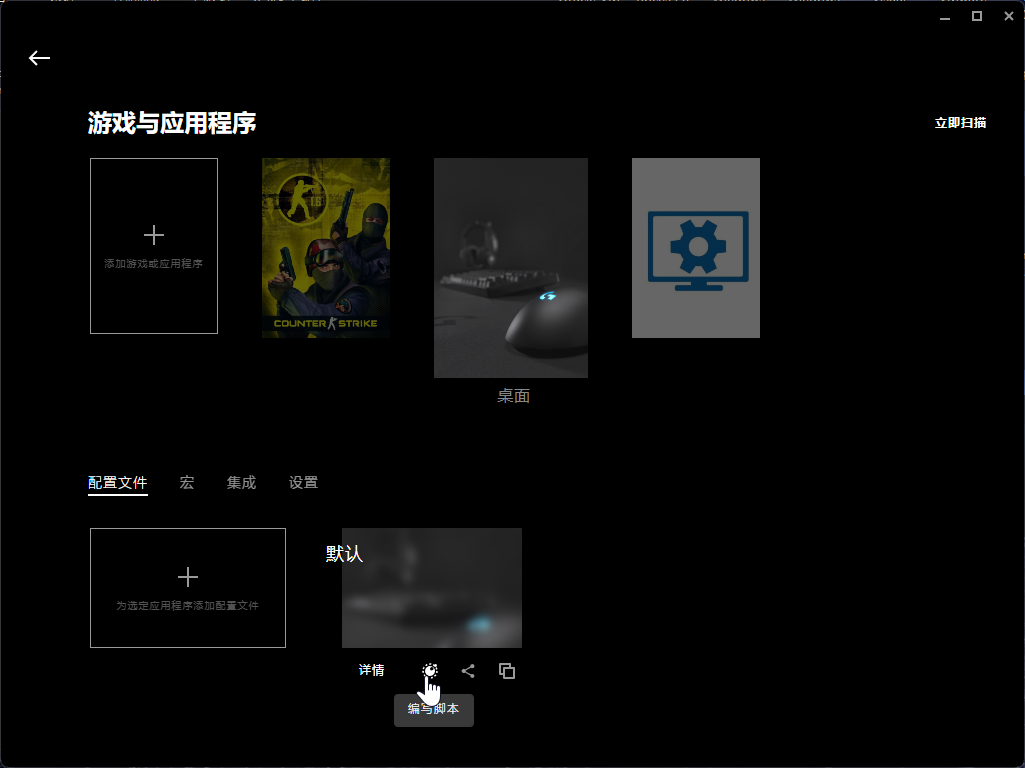
\includegraphics[width=\textwidth]{docs/assets/script.png}
    \caption{点击“编写脚本”}
\end{figure}

点击“脚本-导入”,将 LUA 源文件 \lstinline{main.lua} 导入软件,点击保存并运行。

\begin{figure}[H]
    \Centering
    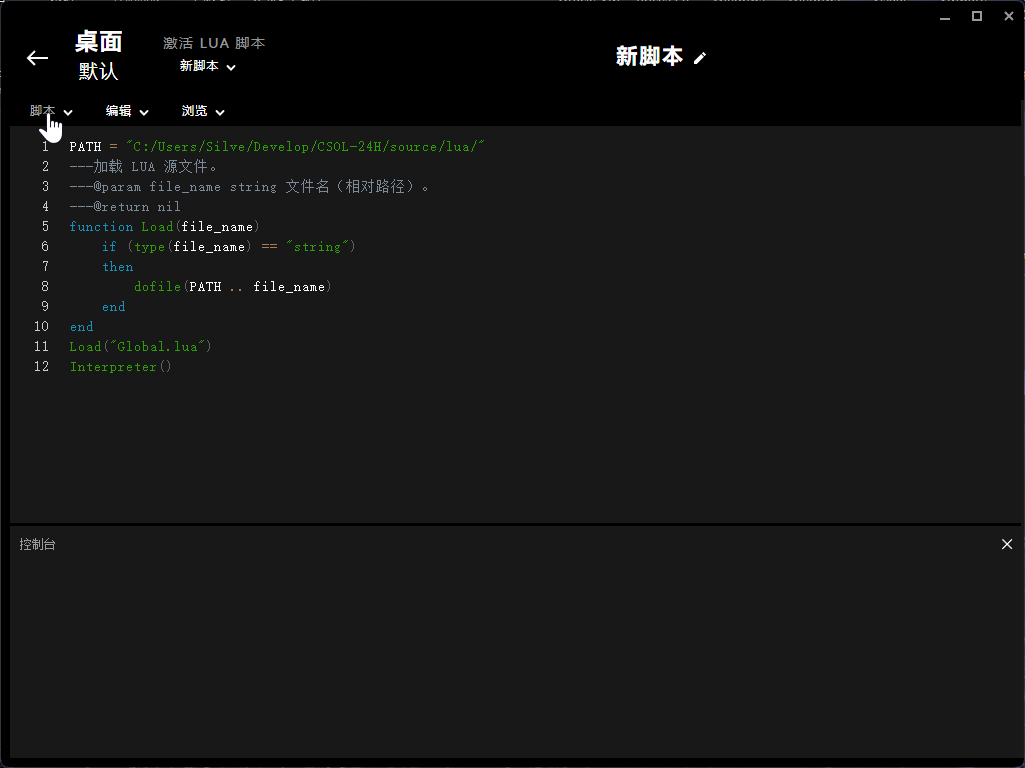
\includegraphics[width=\textwidth]{docs/assets/edit.png}
    \caption{点击“脚本”}
\end{figure}

\begin{figure}[H]
    \Centering
    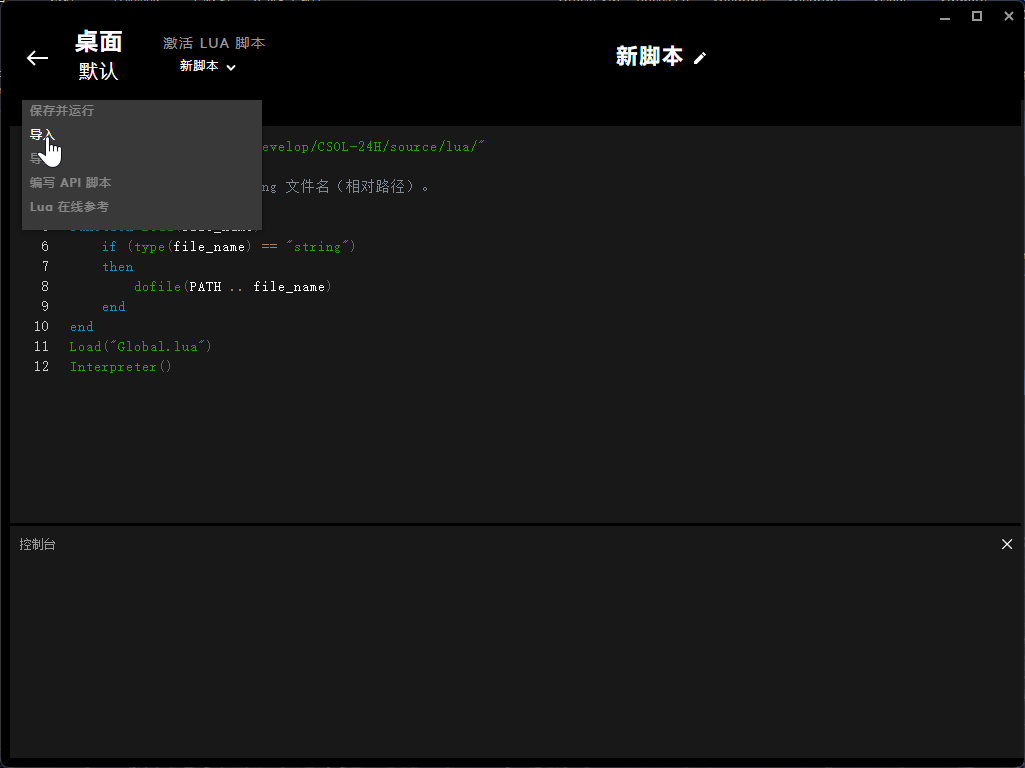
\includegraphics[width=\textwidth]{docs/assets/import.png}
    \caption{点击“导入”}
\end{figure}

\begin{figure}[H]
    \Centering
    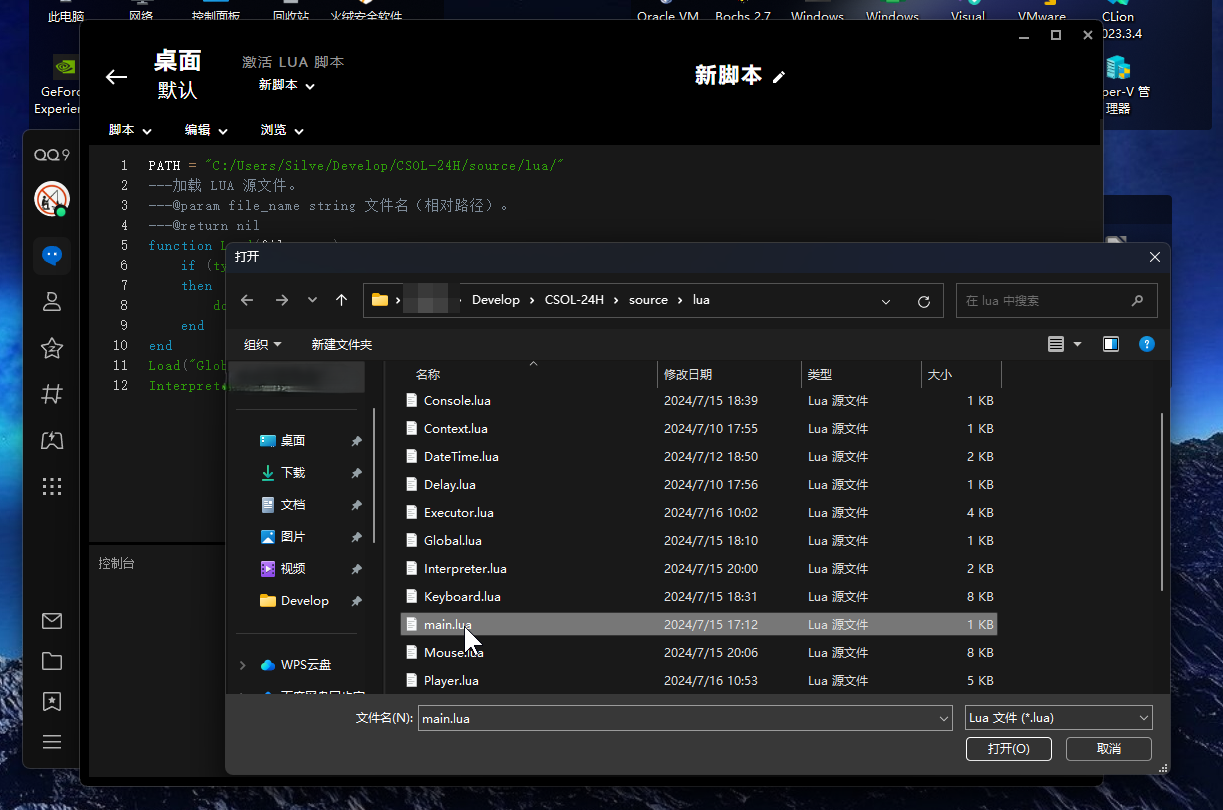
\includegraphics[width=\textwidth]{docs/assets/main.png}
    \caption{选择 \lstinline{main.lua}}
\end{figure}

\begin{figure}[H]
    \Centering
    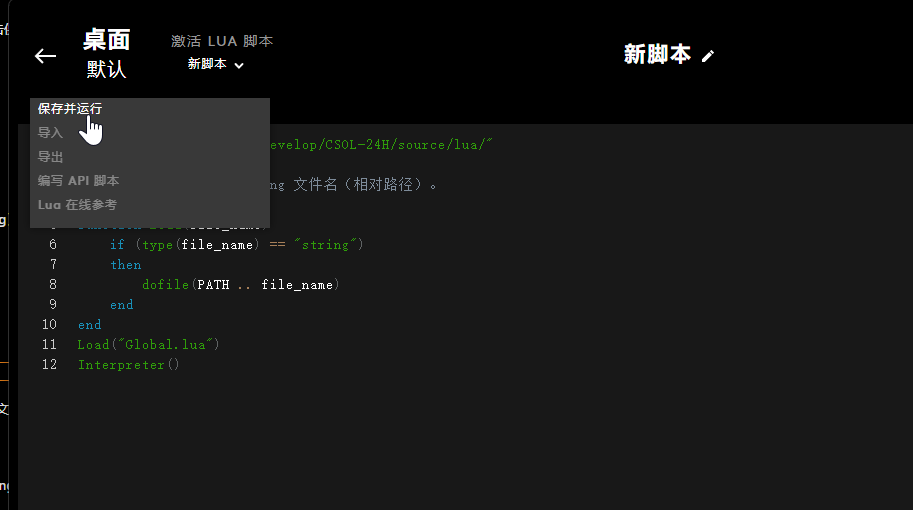
\includegraphics[width=\textwidth]{docs/assets/save_and_run.png}
    \caption{保存并运行}
\end{figure}

看到控制台输出下述文字信息,则说明导入成功。

\begin{figure}[H]
    \Centering
    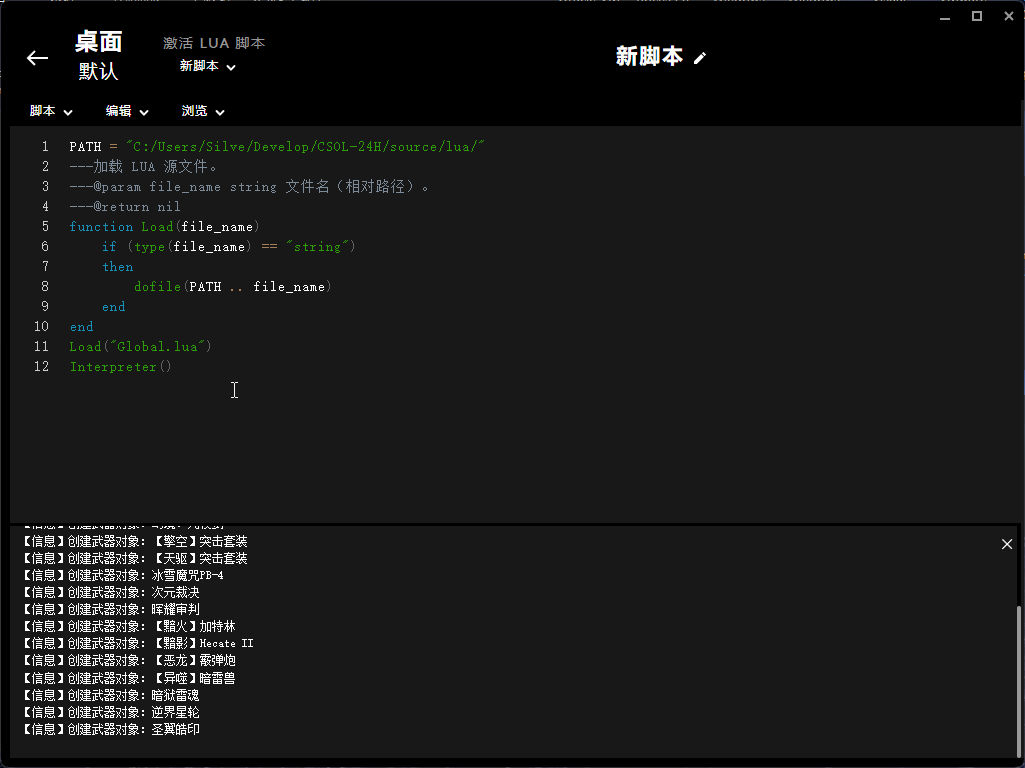
\includegraphics[width=\textwidth]{docs/assets/success.png}
    \caption{保存并运行成功}
\end{figure}

保存并运行后,罗技软件在下一次启动时会自动加载上述脚本文件(启动时加载只会执行一次),无需再重复上述操作。

\textbf{\color{red}但是,加载后若对文件夹内的 LUA 任一个源文件进行修改,则还需要重新在此界面中点击保存并运行。}

\subsection{控制器}

右键在 Powershell 中运行 \lstinline{Controller.ps1},控制器将启动。

\begin{figure}[H]
    \Centering
    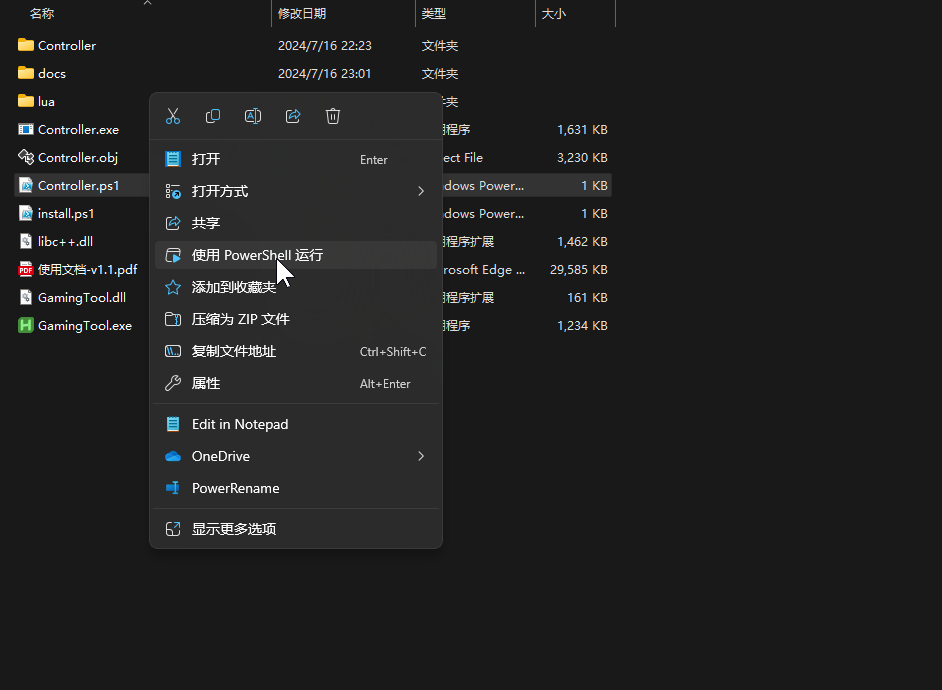
\includegraphics[width=\textwidth]{docs/assets/run_controller.png}
    \caption{运行控制器}
\end{figure}

控制器在 Windows 控制台中运行,在控制台界面中按下 \lstinline{Ctrl} \lstinline{C}(推荐)或直接点击右上角关闭按钮可终止程序。

启动控制器后,会注册如下热键(在阅读完本节之前请先不要尝试):

\begin{itemize}

    \item 0 模式:\lstinline{Ctrl} \lstinline{Alt} \lstinline{Shift} \lstinline{0},启动后的默认模式,该模式下不进行任何操作。

    \item 1 模式:\lstinline{Ctrl} \lstinline{Alt} \lstinline{Shift} \lstinline{1},单武器挂机模式。

    \item 2 模式:\lstinline{Ctrl} \lstinline{Alt} \lstinline{Shift} \lstinline{2},随机武器挂机模式。

    \item 3 模式:\lstinline{Ctrl} \lstinline{Alt} \lstinline{Shift} \lstinline{3},自动合成配件。

    \item 4 模式:\lstinline{Ctrl} \lstinline{Alt} \lstinline{Shift} \lstinline{4},自动重复购买同一件商店物品,可用于批量购买金币道具。

    \item 5 模式:\lstinline{Ctrl} \lstinline{Alt} \lstinline{Shift} \lstinline{5},定位坐标,将结果输出到罗技控制台。

\end{itemize}

控制器会在 \lstinline{lua} 目录下创建临时文件,实时向该临时文件中写入命令,指导 LUA 模块执行相应的操作。
每条命令都有一定的有效期(5 秒),超过有效期的命令不会被 LUA 模块执行。
每条命令的执行完毕都需要一定的时间,\textbf{\color{red}控制器切换模式不会立即停止当前命令的执行,而是有一定的延迟时间}。

\subsection{即时中断功能}

上面提到,控制器切换模式,LUA 模块响应有一定的延迟。
为了使罗技软件能够及时响应紧急的中断消息,本集成工具通过封装罗技 API,在 LUA 模块中引入了即时中断功能。

例如,\textbf{\color{red}若不慎错误地按下前面提及的功能热键,导致鼠标键盘不受控制,可以同时按下键盘上的左 \lstinline{Ctrl} 和右 \lstinline{Ctrl} 紧急暂停,罗技软件会在 10 毫秒内快速响应此中断信号。
紧急暂停后,罗技软件将不再发出任何键鼠操作,直至同时按下键盘上的左 \lstinline{Alt} 和右 \lstinline{Alt} 恢复。}

相应地,您可以在罗技软件控制台中看到相应的提示信息。

\begin{figure}[H]
    \Centering
    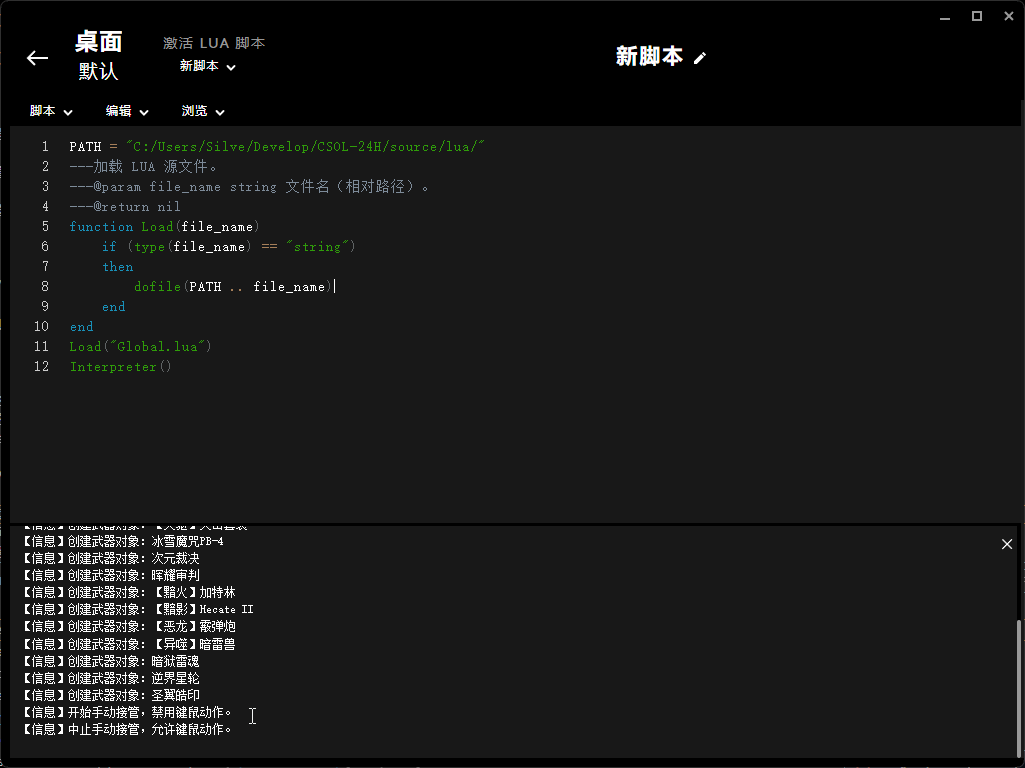
\includegraphics[width=\textwidth]{docs/assets/interrupt.png}
    \caption{即时中断功能提示信息}
\end{figure}

需要注意,紧急暂停功能完全独立于控制器。
\textbf{\color{red}紧急暂停后,控制器仍然会持续向罗技软件下达命令,只是罗技软件并不会执行这些命令。}若要取消当前控制器启用的模式,请按热键将控制器切换回 0 模式。

\subsection{使用 GamingTool}

双击运行解压目录下的 \lstinline{GamingTool.exe}。

有关 GamingTool 使用方法,参考 \href{https://gitee.com/silver1867/gaming-tool}{GamingTool 项目链接}。

\subsection{配置文件}

\lstinline{lua} 目录下的 \lstinline{Setting.lua} 及 \lstinline{WeaponList.lua} 是根据用户自身情况自行定义的配置文件。
按照本文档介绍的方式配置完毕能够正常使用后,您应当妥善保管。
后续版本更新不会对这两个配置文件内容作出较大的变动。
更新到新版本时,只需要将这两份文件原样复制到新版本的 \lstinline{lua} 目录下,并在新版本目录下重新运行一次 \lstinline{install.ps1},在罗技软件中将 \lstinline{main.lua} 重新保存并运行即可。

\subsection{更新方法(初次安装使用可跳过)}

\textbf{\color{red}关闭旧版本控制器和 GamingTool。}

下载新版本压缩包。

\textbf{\color{red}将您在旧版中使用的 \lstinline{Setting.lua} 和 \lstinline{WeaponList.lua} 备份。}

打开新版本 \lstinline{lua} 目录下的 \lstinline{Setting.lua} 和 \lstinline{WeaponList.lua},移动到文件末尾,查看是否有对应版本的更新(更新会注明)。
如有,将新增的部分复制到备份的 \lstinline{Setting.lua} 和 \lstinline{WeaponList.lua} 中并保存。
上述操作完成后,用备份的两个文件\textbf{\color{red}替换}新版本 \lstinline{lua} 目录中的 \lstinline{Setting.lua} 和 \lstinline{WeaponList.lua}。
然后,在新版路径下右键在 Powershell 中运行 \lstinline{install.ps1},并在罗技软件中导入新版 \lstinline{lua} 路径下的 \lstinline{main.lua} 文件,然后点击保存并运行。
随后,运行控制器和 GamingTool,按照本文所述操作方式即可正常使用各项功能。

解压新版本压缩包\textbf{\color{red}(解压路径不能包含非英文字符)},将上述两个文件复制到新版本 \lstinline{lua} 路径下,覆盖其中的 \lstinline{Setting.lua} 和 \lstinline{WeaponList.lua}。

在新版本解压路径下右键在 Powershell 中运行 \lstinline{install.ps1}。

然后,阅读更新说明,向 \lstinline{Setting.lua} 和 \lstinline{WeaponList.lua} 中追加新内容(原有内容保持不变)。

修改完成后,打开罗技软件,导入并运行新版本 \lstinline{lua} 目录下的 \lstinline{main.lua} 文件。